\chapter{Hardware}
%http://samurai1967.dyndns.org/avr-net-io.html
%http://www.fhemwiki.de/wiki/AVR-NET-IO
%http://www.mikrocontroller.net/articles/AVR_Net-IO_Bausatz_von_Pollin
\section{AVR Net-IO-Board}
\begin{figure}[h]
\centering
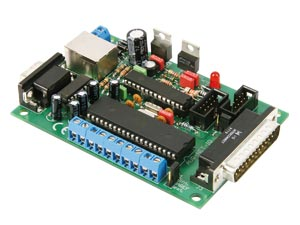
\includegraphics[width=10cm]{content/pictures/avr-net-io.jpg}
\caption{AVR-NET-IO - Pollin GmbH}
%http://www.pollin.de/shop/dt/MTQ5OTgxOTk-/Bausaetze_Module/Bausaetze/Bausatz_AVR_NET_IO.html
\label{fig:B3}
\end{figure}

\subsection{Technische Daten}
\begin{itemize}
  \item Betriebsspannung 9V
  \item Stromaufnahme ca. 190 mA
  \item 8 Digitale Ausgänge, 4 Digitale Eingänge
  \item 4 Analoge Eingänge
  \item ATmega32 Mikrocontroller
  \item integrierte ISP-Schnittstelle
\end{itemize}

\section{Mikrocontroller}
\subsection{ATmega32}

\subsection{ATmega644P}

\subsection{ATmega1284P}

\section{Fuse Bits}

%TODO Wahl der Fuse Bits
